\teory % Структурный элемент: ТЕОРИЯ

Кластеризация (или кластерный анализ) — это задача разбиения множества объектов на группы, называемые кластерами. Внутри каждой группы должны оказаться «похожие» объекты, а объекты разных группы должны быть как можно более отличны. Главное отличие кластеризации от классификации состоит в том, что перечень групп четко не задан и определяется в процессе работы алгоритма
Применение кластеризация в общем виде сводится к следующим этапам:
\begin{enumerate}[label=\arabic*.]
\item Отбор выборки объектов для кластеризации.

\item Определение множества переменных, по которым будут оцениваться объекты в выборке. При необходимости – нормализация значений переменных.

\item Вычисление значений меры сходства между объектами.

\item Применение метода кластерного анализа для создания групп сходных объектов (кластеров).
	
\item Представление результатов анализа
		
	\end{enumerate}

Кластеризация может быть либо непересекающейся (жёсткой), либо пересекающейся. В пересекающейся кластеризации один и тот же документ может принадлежать к нескольким кластерам, в то время как при жёсткой кластеризации каждый документ попадает только в один кластер.

Кластеризация отличается от классификации документов. В классификации классы (и их характеристики) известны заранее, и документы просто распределяются по этим классам. В кластеризации количество, свойства и состав классов заранее неизвестны. Таким образом, классификация — это пример обучения с учителем, а кластеризация — обучения без учителя.

Кластеризация документов делится на две основные подкатегории: жёсткая (hard clustering) и мягкая (soft clustering). Мягкая кластеризация, также известная как пересекающаяся, далее подразделяется на:

    

\begin{itemize}
    \item Жёсткая кластеризация:
    Каждый документ жёстко назначается одному кластеру — формируются непересекающиеся кластеры;

    \item Мягкая кластеризация (Soft/Overlapping):
    Документ может входить сразу в несколько кластеров. Например, документ о «естественном языке и информационном поиске» может быть отнесён к обоим кластерам — «Естественный язык» и «Информационный поиск»;
     \item Разделяющая кластеризация (Partitioning):
    Делит документы на фиксированное количество непустых кластеров. Самый известный метод — K-средних (K-means) и его варианты [4]. Алгоритм начинается с случайного распределения объектов по кластерам, затем в каждой итерации пересчитываются центры (средние) кластеров, и объекты перераспределяются по ближайшим центрам. Алгоритм завершается, когда перераспределение прекращается;
     \item Иерархическая кластеризация (Hierarchical)
    Строит дендрограмму — дерево кластеров, где листья — подмножества документов. Примеры: Иерархическая агломеративная кластеризация (HAC) и метод UPGMA;
     \item Кластеризация на основе частых наборов признаков (Frequent itemset-based):
   Эти методы используют часто встречающиеся наборы признаков (itemsets), извлечённые с помощью ассоциативных правил, для кластеризации документов. Это снижает размерность признаков и улучшает точность и масштабируемость алгоритмов. Дополнительно, каждый кластер можно обозначить частыми наборами терминов.
\end{itemize}


   
В этой категории метки классов (кластеров) не предоставляются. Алгоритм самостоятельно выявляет закономерности и структуры в данных, группируя похожие образцы на основе сходства признаков без предварительного знания о принадлежности к группам. Обычно общее количество кластеров в наборе данных заранее неизвестно. Примеры алгоритмов в этой категории включают K-Means, DBSCAN (Density-Based Spatial Clustering of Applications with Noise) и Fuzzy C-Means (FCM).


Изначально кластеризация документов изучалась с целью повышения точности и полноты (precision и recall) в системах информационного поиска. Также кластеризация используется для автоматического построения иерархических кластеров документов.
Существуют основные сферы применения кластеризации данных:
\begin{itemize}
   \item \textbf{Обнаружение тем (Topic Discovery)}:
       Позволяет выявить скрытые темы и тенденции в больших коллекциях документов;
    \item \textbf{Автоматическая организация контента}:
       Используется для структурирования и классификации информации в новостных сайтах, блогах, корпоративных порталах и цифровых библиотеках;
    \item \textbf{Информационный поиск (Information Retrieval)}:
       Кластеризация помогает группировать документы по темам, повышая релевантность выдачи и упрощая пользователям поиск нужной информации;
    \item \textbf{Мягкая кластеризация (Soft/Overlapping)}:
        Документ может входить сразу в несколько кластеров. Например, документ о «естественном языке и информационном поиске» может быть отнесён к обоим кластерам — «Естественный язык» и «Информационный поиск»;
    \item \textbf{Рекомендательные системы}:
    Позволяет выявить скрытые темы и тенденции в больших коллекциях документов.  ;
    \item \textbf{Автоматическая организация контента}:
       Кластеры документов могут быть использованы для создания кратких тематических сводок;
    \item \textbf{Анализ мнений и отзывов}:
    Помогает в группировке отзывов пользователей по схожим аспектам или эмоциональной окраске;
    \item \textbf{Управление знаниями (Knowledge Management)}:
    В корпоративных системах — для организации внутренних документов, отчетов и технической документации.
\end{itemize}
\section{Алгоритмы кластеризации}
    
\subsection{K MEANS}

Это один из самых популярных методов кластеризации, используемых в машинном обучении. В отличие от обучения с учителем, обучающие данные, которые использует этот алгоритм, не размечены, то есть точки данных не имеют заранее определённой структуры классификации.

Существует множество типов алгоритмов кластеризации, включая эксклюзивную, перекрывающуюся, иерархическую и вероятностную. Алгоритм кластеризации k-средних (k-means) является примером эксклюзивной или «жёсткой» кластеризации. Такая форма группировки предполагает, что каждая точка данных может принадлежать только одному кластеру. Этот тип кластерного анализа широко применяется в области анализа данных для сегментации рынка, кластеризации документов, сегментации изображений и сжатия изображений. Алгоритм k-средних популярен благодаря своей эффективности, простоте и высокой производительности.

Алгоритм k-средних — это итеративный алгоритм кластеризации, основанный на центроидах. Он разбивает набор данных на группы по признаку схожести, определяемой расстоянием до центроида. Центроид (или центр кластера) представляет собой среднее или медианное значение всех точек в кластере — в зависимости от характеристик данных.

Кластеризация методом k-средних представляет собой итеративный процесс минимизации суммы расстояний между точками данных и центроидами соответствующих кластеров.

\begin{equation}
V = \sum_{i=1}^{k} \sum_{x \in S_i} (x - \mu_i)^2,
\end{equation}

где:
\begin{itemize}

\item $k$ — число кластеров;
\item $S_i$ — полученные кластеры;
\item $i = 1,2,\ldots$;
\item $\mu_i$ — центры масс всех векторов из кластера.
\end{itemize}


Алгоритм кластеризации k-средних работает путём категоризации точек данных в кластеры на основе математической меры расстояния — обычно евклидовой — до центра кластера. Цель — минимизировать сумму расстояний между точками данных и их соответствующими центроидами. Точки данных, ближайшие к центроиду, группируются в одну категорию. Более высокое значение k (число кластеров) означает меньшие по размеру, но более детализированные кластеры; более низкое значение k — более крупные кластеры с меньшей детализацией.

Следующий шаг включает в себя двухэтапный итерационный процесс, основанный на алгоритме машинного обучения ожидания-максимизации. На этапе ожидания каждая точка данных присваивается ближайшему центроиду на основе расстояния (обычно евклидова). На этапе максимизации вычисляется среднее значение всех точек для каждого кластера и пересчитывается центр кластера — центроид. Этот процесс повторяется до тех пор, пока положения центроидов не стабилизируются (сойдутся) или не будет достигнуто максимальное количество итераций.

Алгоритм кластеризации K-средних прост, но чувствителен к начальным условиям и выбросам. Важно оптимизировать инициализацию центроидов и количество кластеров k, чтобы получить максимально информативные кластеры. 

Ввиду этого я выбрал более подходящих алгоритм кластеризации в своей работает - HDBSCAN.

\subsection{HDBSCAN}
HDBSCAN основан на DBSCAN, поэтому стоит рассказать сначала о нем.

Алгоритм DBSCAN — это классический метод кластеризации на основе плотности, который эффективно определяет шумовые (выбросные) точки. Он рассматривает кластеры как наибольшие множества данных, связанных плотностью, и основным принципом является то, что точки, принадлежащие одному кластеру, связаны друг с другом через плотность.

Алгоритм DBSCAN был впервые предложен Эстером и соавторами. Каждая точка данных в кластере должна иметь в своём окрестности (радиусе Eps) как минимум заданное количество точек (MinPts). 

Алгоритм DBSCAN использует итерационные запросы для выполнения кластеризации. Сначала, на основе заданных параметров Eps и MinPts, определяется множество всех основных (ядровых) точек в наборе данных — оно называется множеством N. Затем рассматривается основная точка o из набора данных. Если точка o ещё не отнесена к какому-либо кластеру, создаётся новый кластер C, и все точки в окрестности точки o, включая её саму, помечаются как принадлежащие кластеру C.

Далее, если некоторая точка p из окрестности o также является основной, то все точки в её окрестности также добавляются в кластер C. Эти действия повторяются для оставшихся точек кластера C, пока не перестанут добавляться новые точки. Описанный процесс повторяется для всех точек из множества N, которые ещё не были обработаны, до тех пор, пока все основные точки не будут рассмотрены.

Алгоритм DBSCAN последовательно «поглощает» точки, которые находятся в области плотности, напрямую доступной из основной точки p. Если между двумя кластерами существует плотностная связь, они объединяются в один. Это даёт преимущество в обнаружении кластеров произвольной формы и идентификации шумовых точек. Однако, производительность алгоритма по времени может быть низкой из-за необходимости нахождения основных точек и анализа всех остальных.
\begin{figure}[h!]
    \centering
    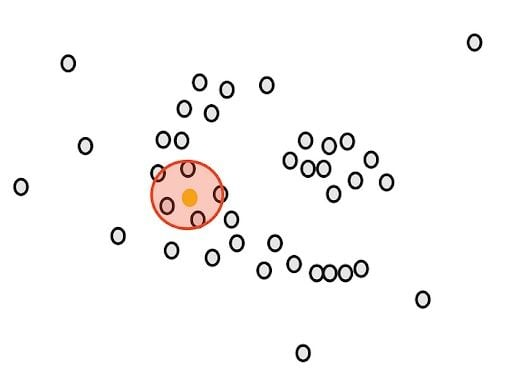
\includegraphics[width=0.7\textwidth]{styles/diploma/inc/dbscan.jpg} % можно .png, .pdf и т.п.
    \caption{Иллюстарция работы алгоритма DBSCAN}
    \label{fig:example}
\end{figure}

В свою очередь отличительным признаком  HDBSCAN является то, что он не выбирает кластеры на основе глобального порога epsilon, а создаёт иерархию для всех возможных значений epsilon с учётом параметра minPts как минимального размера кластера.
\subsubsection{Расстояние взаимной достижимости}
В HDBSCAN ядровое расстояние (dcore) определяется как расстояние от объекта до его minPts-ближайшего соседа. Построенная иерархия основана на взаимном достижимом расстоянии, которое для двух объектов $x_p$ и $x_q$ определяется как:

\begin{equation}
\max\{d_{\text{core}}(x_p),\ d_{\text{core}}(x_q),\ d(x_p, x_q)\} ,
\end{equation}
где:
\begin{itemize}
\item  $d(x_p, x_q)$ — обычное расстояние между объектами, например, евклидово. 
\end{itemize}

Такой подход отделяет разреженные точки от остальных хотя бы на их ядровое расстояние и делает кластеризацию устойчивее к шуму.





Набор данных можно представить в виде графа, где объекты — это вершины, соединённые рёбрами с весами, равными взаимному достижимому расстоянию. Построив по этому графу минимальное остовное дерево и отсортировав его рёбра по mutual reachability, формируется иерархическое дерево (дендрограмма). Задав значение epsilon как уровень горизонтального сечения и выбрав все кластеры, содержащие не менее minPts точек на этом уровне плотности, можно извлечь кластеры DBSCAN для этого epsilon из иерархии.

\subsubsection{Сжатая иерархия кластеров}

Поскольку HDBSCAN направлен на обнаружение кластеров с различной плотностью, он строит упрощённую версию сложного иерархического дерева — сжатое дерево кластеров. Этот подход следует концепции обрезки дерева, которая имеет много вариантов в литературе, таких как обрезка мелких кластеров (runt pruning) по Штюцле или обрезка дерева, построенного с помощью устойчивого алгоритма одиночной связи по Чаудхури и др.

Начиная с корня, HDBSCAN рассматривает разделение кластера как истинное только в том случае, если оба дочерних кластера содержат не менее minPts объектов. Если оба содержат меньше minPts, считается, что кластер исчез на этом уровне плотности. Если только один из дочерних кластеров содержит меньше minPts, считается, что родительский кластер просто потерял точки, но всё ещё существует. "Потерянные" точки считаются шумом. Этот процесс упрощения приводит к иерархии возможных кластеров на разных уровнях плотности.


\subsubsection{Выбор кластеров на основе стабильности}

Имея сжатое дерево кластеров, один из возможных подходов — просто выбрать все листовые узлы. Это кластеры с наименьшими значениями epsilon в иерархии, которые больше нельзя разделить с учётом параметра minPts. Этот метод выбора — один из двух вариантов, реализованных в Python-библиотеке HDBSCAN, и далее будет называться HDBSCAN(leaf). Он приводит к формированию мелких, детализированных кластеров.

Имея сжатое дерево кластеров, один из возможных подходов — просто выбрать все листовые узлы. Это кластеры с наименьшими значениями epsilon в иерархии, которые больше нельзя разделить с учётом параметра minPts. Этот метод выбора — один из двух вариантов, реализованных в Python-библиотеке HDBSCAN, и далее будет называться HDBSCAN(leaf). Он приводит к формированию мелких, детализированных кластеров.

Второй вариант — метод eom (excess of mass, избыток массы). Этот метод рекомендуется Кампелло и др. как оптимальное глобальное решение задачи выбора кластеров с наибольшей стабильностью. Он определяет стабильность следующим образом:
\begin{equation}
\begin{aligned}
S(C_i) &= \sum_{x_j \in C_i} \left( \lambda_{\max}(x_j, C_i) - \lambda_{\min}(C_i) \right) \\
       &= \sum_{x_j \in C_i} \left( \frac{1}{\varepsilon_{\min}(x_j, C_i)} - \frac{1}{\varepsilon_{\max}(C_i)} \right)
\end{aligned}
\end{equation}


Значение плотности $\lambda$ при этом принимается равным $\frac{1}{\epsilon}$. Это означает, что значения $\lambda$ возрастают от корня к листьям дерева, в то время как соответствующие значения расстояния $\epsilon$ уменьшаются. Вычитание $\lambda_{min}(C_i)$ — плотностного уровня, на котором кластер $C_i$ впервые появляется, из значения, при котором объект $x_j ∈ C_i$ больше не принадлежит $C_i$, даёт время жизни объекта $x_j$ в кластере. Суммируя времена жизни всех объектов в кластере $C_i$, получают общее время жизни кластера $S(C_i)$, которое называется стабильностью, поскольку кластеры с наибольшим временем жизни считаются наиболее устойчивыми.

Затем формируется задача оптимизации, целью которой является максимизация суммы стабильностей кластеров:
\begin{equation}
\begin{aligned}
\max_{\delta_2, \ldots, \delta_k} \quad & J = \sum_{i=2}^{k} \delta_i S(C_i) \\
\text{subject to} \quad & \delta_i \in \{0,1\}, \quad i = 2, \ldots, k \\
& \sum_{j \in I_h} \delta_j = 1, \quad \forall h \in \mathbf{L}
\end{aligned}
\end{equation}


где:
\begin{itemize}
    \item $L = \{h \mid C_h \text{ — листовой кластер}\}$;
    \item $I_h$ — множество кластеров на пути от листьев к исключённому корню;
    \item $\delta_i$ — булевый индикатор того, выбран ли соответствующий кластер.
\end{itemize}

 Определение (4) гарантирует, что на любой ветви от листа к корню может быть выбран не более одного кластера.

Для решения этой задачи алгоритм выбора кластеров HDBSCAN проходит дерево снизу вверх. Значение стабильности каждой вершины сравнивается с суммой стабильностей её вложенных подкластеров. Таким образом, стабильности распространяются и обновляются при подъёме по дереву до тех пор, пока на каждой ветке не будет найден и выбран кластер с наивысшей стабильностью.
\subsubsection{Подход для оптимального выбора кластеров}

Метод извлечения кластеров на основе избыточной массы (eom), описанный выше, соответствует обобщённой концепции «Framework for Optimal Selection of Clusters» (FOSC), предложенной Кампелло и соавт.

FOSC требует соблюдения двух ключевых свойств:

Во-первых, выбранная мера для отбора кластеров — в данном случае критерий стабильности — должна быть локальной, то есть её можно вычислить для каждого кластера независимо от других выбранных кластеров.

Во-вторых, она должна быть аддитивной, то есть должно иметь смысл суммировать значения, вычисленные для кластеров (в данном случае — стабильности кластеров), чтобы можно было сформулировать задачу оптимизации как задачу максимизации суммы этих значений.

Кроме того, необходимо обеспечить, чтобы на каждой ветви иерархического дерева был выбран ровно один кластер. Эта формализованная задача затем может быть решена путём обхода иерархического дерева снизу вверх, начиная с листьев, принимая решение по каждому кандидату — включать его в финальное решение или нет.

Таким образом, FOSC предоставляет эффективный способ нахождения глобально оптимального решения для извлечения кластеров на основе выбранной меры.

После выделения стабильных кластеров с помощью HDBSCAN становится возможным выявлять устойчивые структуры в данных, даже если они отличаются по плотности или имеют сложную форму. Однако, чтобы кластеризация была действительно эффективной при работе с высокоразмерными или текстовыми данными, необходим предварительный этап — преобразование исходной информации в векторное представление, известное как эмбединги..

В обработке естественного языка эмбединги слов представляют собой числовое представление слов. Эти встраивания используются при анализе текста. Как правило, это векторы с действительными значениями, которые кодируют значение слова таким образом, что слова, находящиеся ближе друг к другу в векторном пространстве, считаются схожими по смыслу [1]. Эмбединги можно получить с помощью моделей языка и методов извлечения признаков, при которых слова или фразы из словаря отображаются в векторы действительных чисел.

Таким образом, эмбединги служат мостом между необработанными (сырьёвыми) данными и алгоритмами кластеризации: они превращают сложные, разнородные данные в числовое представление, с которым могут работать методы вроде HDBSCAN, выявляя скрытые паттерны, структуры и смысловые группы.



